\documentclass{article}

\usepackage[utf8]{inputenc}
\usepackage[spanish]{babel}

\usepackage{caratula}
\usepackage[toc,page]{appendix}
\usepackage{subcaption}
\usepackage{graphicx}
\usepackage{dirtytalk}
\usepackage{enumerate}

\usepackage{amssymb}
\usepackage{mathtools}
\usepackage{amsmath}
\usepackage{amsthm}

\usepackage{algorithm}
\usepackage{algpseudocode}
\usepackage{listingsutf8}

\usepackage{float}
\floatplacement{figure}{h!}

\usepackage{geometry}
\usepackage{fixltx2e}
\usepackage{wrapfig}
\usepackage{cite}
\usepackage{dsfont}
\usepackage{ulem}

\usepackage[space]{grffile}

\geometry{
 a4paper,
 total={210mm,297mm},
 left=30mm,
 right=30mm,
 top=20mm,
 bottom=20mm,
 }

\usepackage{booktabs}

% sql stuff
\usepackage{listings}
\usepackage{courier}
\usepackage{pdflscape}

\newcommand\JSONnumbervaluestyle{\color{blue}}
\newcommand\JSONstringvaluestyle{\color{red}}

% switch used as state variable
\newif\ifcolonfoundonthisline

\makeatletter

\lstdefinestyle{json}
{
  showstringspaces    = false,
  keywords            = {false,true},
  alsoletter          = 0123456789.,
  morestring          = [s]{"}{"},
  stringstyle         = \ifcolonfoundonthisline\JSONstringvaluestyle\fi,
  MoreSelectCharTable =%
    \lst@DefSaveDef{`:}\colon@json{\processColon@json},
  basicstyle          = \ttfamily,
  keywordstyle        = \ttfamily\bfseries,
}

% flip the switch if a colon is found in Pmode
\newcommand\processColon@json{%
  \colon@json%
  \ifnum\lst@mode=\lst@Pmode%
    \global\colonfoundonthislinetrue%
  \fi
}

\lst@AddToHook{Output}{%
  \ifcolonfoundonthisline%
    \ifnum\lst@mode=\lst@Pmode%
      \def\lst@thestyle{\JSONnumbervaluestyle}%
    \fi
  \fi
  %override by keyword style if a keyword is detected!
  \lsthk@DetectKeywords%
}

% reset the switch at the end of line
\lst@AddToHook{EOL}%
  {\global\colonfoundonthislinefalse}

\newtheorem{theorem}{Teorema}[section]
\newtheorem{corollary}{Corolario}[theorem]
\newtheorem{lemma}{Lema}[theorem]

\theoremstyle{definition}
\newtheorem{definition}{Definición}[section]

\theoremstyle{remark}
\newtheorem*{remark}{Observación}

\usepackage[dvipsnames]{xcolor}

% table of contents depth
\setcounter{tocdepth}{3}

\begin{document}
% Estos comandos deben ir antes del \maketitle
\materia{Ingeniería de Software II} % obligatorio

\titulo{TP2}
\subtitulo{Alerta y Vigliancia de Yacimientos Semi-Automático \\ \textbf{AVYSA} \\ \today}
\grupo{}

\integrante{Christian Cuneo}{755/13}{chriscuneo93@gmail.com}
\integrante{Federico Beuter}{827/13}{federicobeuter@gmail.com}
\integrante{Mauro Cherubini}{835/13}{cheru.mf@gmail.com}
\integrante{Mario Ezequiel Ginsberg}{145/14}{ezequielginsberg@gmail.com}
\integrante{Martín Baigorria}{575/14}{martinbaigorria@gmail.com}

\maketitle

\tableofcontents

\vspace{2cm}

\begin{figure}[H]
    \centering
    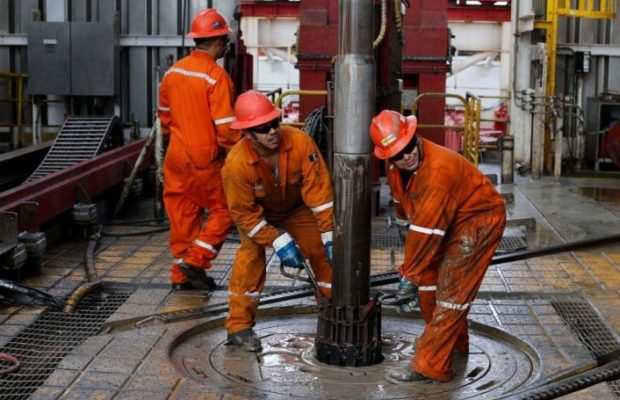
\includegraphics[scale=0.6]{figures/trabajadores.jpg}
    \caption{Trabajadores arreglando un problema diagnosticado mediante el sistema ARS luego del segundo recuperatorio.}
\end{figure}

\pagebreak

\section{Introducción}

Luego de desarrollar el simulador SimOil, aprovechando que ya habíamos adquirido el conocimiento de dominio de la industria petrolera, el Ministerio de Energía se ha mostrado interesado en integrar dicho sistema de simulación al sistema de control de pozos inteligentes que posee la empresa petrolera estatal. Este sistema monitorea el flujo producido, el flujo de reinyección de gas/agua, las presiones y las temperaturas por pozo. De esta manera, se pueden diagnosticar problemas y gestionar mejor los recursos de cada yacimiento. La tecnología de pozos inteligentes utiliza una serie de sensores ubicados en cada pozo, que reportan datos de alta frecuencia. Dado el gran volumen de datos, los ingenieros requieren un sistema diseñado especialmente para identificar cualquier tipo de inconveniente a partir del estado de los pozos.

Para poder integrar el sistema SimOil al sistema de control de pozos inteligentes, la solución planteada busca en primer lugar reducir la dimensionalidad de los datos de alta frecuencia para que los mismos sean mas simples de procesar a través de un sistema automatizado de supervisión de yacimiento denominado ARS. El sistema ARS luego preparara los datos almacenados para que luego puedan ser utilizados por los diferentes ingenieros de forma remota. A grandes rasgos, el sistema consistirá en un pipeline de tres etapas:

\begin{figure}[H]
  \resizebox{\textwidth}{!}{
    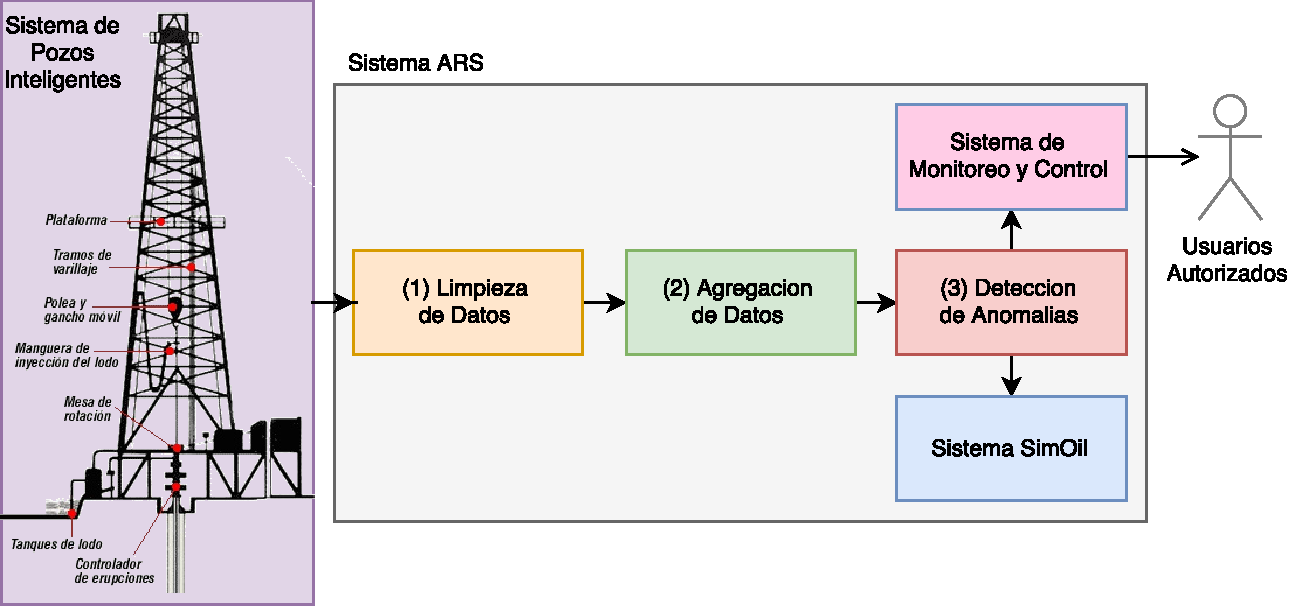
\includegraphics[scale=1]{figures/pipeline.pdf}
  }
  \caption{Esquema ilustrativo del sistema. El sistema de pozos inteligentes provee los datos de alta frecuencia a partir de sensores, que son procesados por el sistema ARS. A grandes rasgos, el sistema consiste en un pipeline de tres etapas, el cual luego provee datos a los ingenieros.}
\end{figure}

Cada uno de estos módulos del pipeline tiene las siguientes características:
\begin{enumerate}
	\item Limpieza de datos: Dado que los datos producidos por los sensores pueden no ser realistas, los mismos se filtran antes de comenzar con su correspondiente procesamiento. Los especialistas del dominio nos han confirmado que es posible identificar aproximadamente un 80\% de las anomalías utilizando limites superiores e inferiores para las diferentes medidas.
	\item Agregación de datos: El proceso de agregación transforma los datos de alta frecuencia en intervalos manejables de 15 minutos. Es razonable pensar que el estado de las variables de cada pozo es relativamente estable en intervalos lo suficientemente chicos, por lo que no tiene sentido procesar todas las mediciones de forma individual.
	\item Detección de anomalías: Utilizando los datos procesados y agregados, en conjunto con las simulaciones provistas por el sistema SimOil, es posible detectar problemas en pozos individuales utilizando algoritmos de Machine Learning. Las diferentes anomalías detectadas son luego reportadas al Jefe de Operaciones del respectivo yacimiento mediante SMS. Estos datos también están disponibles para que otros usuarios autorizados los consulten mediante una interfaz web.
\end{enumerate}

Al detectarse una anomalía, también se genera una alarma sonora en el centro de control del respectivo yacimiento donde sucedió el problema. Las alarmas pueden ser deshabilitadas de forma manual o mediante la interfaz del sistema ARS. Para que el sistema vuelva a operar de forma normal, el Jefe de Operaciones debe tomar una acción correctiva de ser necesaria o reportar un falso positivo de la alarma.

Dado que las normas internacionales son muy estrictas, se requiere que todos los registros de anomalías sean almacenados e informados a organismos certificadores de calidad, como el Ente Regulador de Seguridad Medio Ambiental (ERSMA). Los formularios de eventos deben estar disponibles para el Ministerio y para el Ente Regulador en todo momento. En cuanto a la accesibilidad de los datos y los reportes, el sistema también debe contar con perfiles de usuarios según sus cargos y responsabilidades.

El costo de construir un yacimiento petrolero es considerable. Cualquier decisión que no se tome de forma correcta puede tener un gran costo para el Ministerio. Por esta razón se considera que los datos son muy sensibles, haciendo necesario el almacenamiento de los mismos en un sitio seguro con un sistema de backup en caso de perdida o siniestro.

A modo de resumen, el ministerio ha puesto especial énfasis en las siguientes funcionalidades y atributos de calidad:
\begin{enumerate}
	\item Control de acceso diferenciado según el perfil del usuario.
	\item Tolerancia a fallas.
	\item Manejo de grandes volúmenes de datos.
	\item Seguridad a nivel de usuarios y acceso a datos.
	\item Gestión de las alarmas, formularios e informes de eventos críticos.
	\item Acceso al sistema de monitoreo y control desde el Ministerio.
	\item Acceso al sistema de informes de eventos críticos desde los entes reguladores.
	\item Toda la información estará centralizada dentro del Ministerio. El sistema no debe tener ningún tipo de demoras, en especial en las búsquedas de eventos, y debe tener una alta disponibilidad. Se debe buscar un mecanismo para que las consultas recurrentes sean rápidas. Esto podría implementarse mediante caching.
\end{enumerate}

\section{Casos de uso} \label{cu}

\subsection{Diagrama}

\begin{figure}[H]
    \centering
    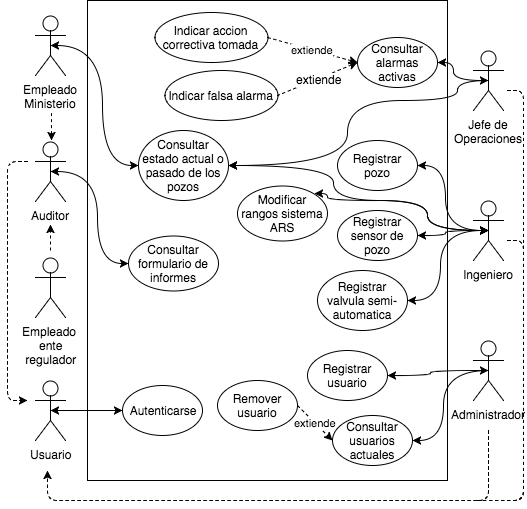
\includegraphics[width=0.7\textwidth]{figures/casosuso.png}
    \caption{Diagrama de casos de uso}
    \label{fig:casosuso}
\end{figure}

\subsection{Descripción}

\begin{enumerate}
    \item \textbf{Autenticándose}: La primera acción que tiene que realizar cualquier usuario, no importe su perfil, para poder seguir interactuando con el sistema con los permisos que tenga su perfil.
    \item \textbf{Registrando usuario}: La forma que tiene el administrador de ingresar un nuevo usuario al sistema, indicando el perfil que va a utilizar.
    \item \textbf{Removiendo usuario}: El administrador le saca el acceso al sistema a un usuario en particular.
    \item \textbf{Consultando usuarios actuales}: El administrador lista los usuarios actuales.
    \item \textbf{Registrando pozo}: De esta forma el ingeniero hace que el sistema considere un nuevo pozo en su procesamiento y lo agregue al simulador de simoil entre otras cosas.
    \item \textbf{Registrando sensor de pozo}: El ingeniero registra un nuevo sensor indicando el pozo al que pertenece para que el sistema sepa a que pozo pertenece.
    \item \textbf{Registrando válvula semiautomática}: El ingeniero registra una nueva válvula semiautomática indicando el pozo al que pertenece y su función.
    \item \textbf{Modificando rangos de sistema ARS}: Se modifican los rangos de limpieza de datos.
    \item \textbf{Consultando estado actual o pasado de los pozos}: Para consultar una historia de los valores de los sensores, posiciones de las válvulas y estados de alerta para cada pozo.
    \item \textbf{Consultando formulario de informes}: Se listan los informes detallados de eventos detectados por el sistema.
    \item \textbf{Consultando alarmas activas}: De esta forma el jefe de operaciones tiene acceso a las alarmas activas.
    \item \textbf{Indicando falsa alarma}: El jefe de operaciones cierra una alarma indicando que fue falsa alarma.
    \item \textbf{Indicando acción correctiva tomada}: El jefe de operaciones cierra una alarma indicando la acción correctiva tomada.
\end{enumerate}

\subsection{Especificación}

\newcommand{\curef}[1]{\textbf{Caso de uso \ref{cu:#1}}}
\newcommand{\cutitle}[1]{\renewcommand{\givencutitle}{#1}}
\newcommand{\cuactors}[1]{\renewcommand{\givencuactors}{#1}}
\newcommand{\cupre}[1]{\renewcommand{\givencupre}{#1}}
\newcommand{\cupost}[1]{\renewcommand{\givencupost}{#1}}
\newcommand{\cucourse}[1]{\renewcommand{\givencucourse}{#1}}
\newcommand{\culabel}[1]{\renewcommand{\givenculabel}{#1}}
\newcommand{\cucaption}[1]{\renewcommand{\givencucaption}{#1}}
\newcommand{\givencutitle}{REQUIRED!}
\newcommand{\givencuactors}{REQUIRED!}
\newcommand{\givencupre}{-}
\newcommand{\givencupost}{-}
\newcommand{\givencucourse}{REQUIRED!}
\newcommand{\givenculabel}{REQUIRED!}
\newcommand{\givencucaption}{} % optional

\newenvironment{casodeuso}
{\begin{table}[H]}{%
\begin{tabular}{|p{0.5\linewidth} p{0.5\linewidth}|}\hline
\multicolumn{2}{|l|}{\textbf{Caso de Uso: \ref{cu:\givenculabel}) \givencutitle}} \\
\multicolumn{2}{|l|}{\textbf{Actor:} \givencuactors} \\
\multicolumn{2}{|l|}{\textbf{Pre:} \givencupre} \\
\multicolumn{2}{|l|}{\textbf{Post:} \givencupost} \\
\vspace{1px}\textbf{Curso Normal} & \vspace{1px}\textbf{Curso Alternativo} \\
\givencucourse
\hline
\end{tabular}
\caption{\givencutitle}
\label{cu:\givenculabel}
\end{table}}

En esta sección identificaremos los tres casos de uso principales y los especificaremos en detalle utilizando la tabla de curso normal/alternativo.

\begin{casodeuso}
  \cutitle{Registrando válvula semiautomática}
  \cuactors{Ingeniero}
  \cupre{Ingeniero esta autenticado}
  \cupost{Válvula y su información queda registrada en el sistema para un poso especifico}
  \cucourse{
    1. El ingeniero selecciona la opción de ingresar una válvula & \\
    2. El sistema carga el listado de pozos actuales y sus válvulas \\
    3. El ingeniero selecciona un pozo al que corresponde la válvula & \\
    4. El sistema carga el listado de tipos de válvula & \\
    5. El ingeniero selecciona que tipo de válvula a ingresar & 5.1. La válvula del tipo seleccionado ya fue ingresada para ese pozo. Vuelve a 5. \\
    6. El ingeniero confirma selección & \\
    7. El sistema persiste la válvula & \\
    8. El sistema informa éxito de operación & \\
    9. Fin del caso & \\
  }
  \culabel{regval}
\end{casodeuso}

\begin{casodeuso}
  \cutitle{Indicando acción correctiva tomada}
  \cuactors{Jefe de operaciones}
  \cupre{Jefe de operaciones esta autenticado}
  \cupost{El evento queda cerrado junto con su informe}
  \cucourse{
    1. El jefe de operaciones selecciona la opción de indicar acción correctiva para la alarma seleccionada en la lista de alarmas activas & \\
    2. El sistema carga en detalle la alarma seleccionada & \\
    3. El jefe de operaciones indica de forma detallada la acción tomada & \\
    4. El jefe de operaciones confirma la operación & 4.1 Descripción es muy corta, vuelve a 3\\
    5. El sistema persiste la acción & \\
    6. El sistema completa el informe de la alarma & \\
    7. Fin del caso & \\
  }
  \culabel{indacc}
\end{casodeuso}

\begin{casodeuso}
  \cutitle{Consultando estado actual o pasado de los pozos}
  \cuactors{Empleado del ministerio, Ingeniero o Jefe de Operaciones}
  \cupre{El usuario esta autenticado y tiene el perfil correspondiente}
  \cupost{El usuario accedió a la información del estado de los pozos que necesitaba}
  \cucourse{
    1. El usuario selecciona la opción de listar los pozos & \\
    2. El sistema lista los pozos & \\
    3. El usuario selecciona el pozo a consultar & \\
    4. El sistema encuentra los registros de estados de válvulas para ese pozo & \\
    5. El sistema encuentra los registros de estados de sensores para ese pozo & \\
    6. El sistema encuentra los registros de alertas para ese pozo & \\
    7. El sistema muestra de forma detallada el historial y el estado actual de este pozo & \\
    8. Fin del caso & \\
  }
  \culabel{estact}
\end{casodeuso}

\pagebreak

\section{Atributos de calidad}

Antes de realizar la arquitectura, llevamos a cabo un Quality Attribute Workshop (QAW) para identificar los diferentes atributos de calidad requeridos. En nuestras reuniones con los stakeholders (consultas con el tutor), generamos, priorizamos y refinamos los diferentes atributos. Especificamos estos atributos de calidad mediante escenarios. La priorización final de los atributos de calidad que se acordó fue la siguiente:

\begin{enumerate}
  \item Performance
  \item Disponibilidad
  \item Seguridad
  \item Usabilidad
  \item Modificabilidad
\end{enumerate}

Para cada tipo de atributo de calidad definimos distintos escenarios de acuerdo a lo relevado.

\subsubsection{Performance}

1)
\begin{itemize}
  \item Descripción: La búsqueda de eventos en el sistema debe tardar a lo sumo medio segundo.
  \item Fuente: Auditor.
  \item Estímulo: Escribe en el buscador el evento a buscar y aprieta el botón Buscar.
  \item Artefacto: Sistema de Informes de Eventos.
  \item Entorno: Normal.
  \item Respuesta: Se obtienen los datos del evento buscado. Si la búsqueda es idéntica a otra realizada hace menos de 1 hora, la respuesta llegará más rápido.
  \item Medición: El sistema responderá la búsqueda en menos de 100 ms en el caso de una búsqueda repetida recientemente, y en menos de 500 ms en cualquier otro caso.
\end{itemize}

2)
\begin{itemize}
  \item Descripción: La limpieza de datos deberá remover aproximadamente el 80\% de los picos no realistas del conjunto de datos.
  \item Fuente: Interna. % ó Ingeniero
  \item Estímulo: Llegan nuevos datos a ser limpiados de datos no realistas. % ó Selecciona el conjunto de datos a limpiar y  \item aprieta el botón Limpiar.
  \item Artefacto: Sistema de Procesamiento de Mediciones. % ó Sistema de Monitoreo y Control.
  \item Entorno: Normal.
  \item Respuesta: El sistema realiza la limpieza de datos correctamente.
  \item Medición: Aproximadamente el 80\% de los picos fuera de los límites superior e inferior fueron eliminados del conjunto de datos.
\end{itemize}

3)
\begin{itemize}
  \item Descripción: La detección de anomalías no debe tardar más de 5 minutos.
  \item Fuente: Interna.
  \item Estímulo: Llegan nuevos datos anómalos a ser analizados.
  \item Artefacto: Detector de Anomalías.
  \item Entorno: Normal.
  \item Respuesta: Se detectan las anomalías y se da aviso al Gestor de Anomalías.
  \item Medición: Las anomalías son detectadas en menos de 5 minutos.
\end{itemize}

\pagebreak

4)
\begin{itemize}
  \item Descripción: Ante un pronóstico catastrófico, la alarma debe ser enviada inmediatamente.
  \item Fuente: Interna.
  \item Estímulo: Evento catastrófico detectado por el módulo Detector de Anomalías.
  \item Artefacto: Gestor de Anomalías.
  \item Entorno: Normal.
  \item Respuesta: Envío inmediato de SMS al Jefe de Operaciones del yacimiento.
  \item Medición: El SMS se envía en menos de 50 ms.
\end{itemize}

\subsubsection{Disponibilidad}

1)
\begin{itemize}
  \item Descripción: El sistema de procesamiento de mediciones debe estar en funcionamiento todo el tiempo para garantizar la mayor efectividad de detección de catástrofes.
  \item Fuente: Interna.
  \item Estímulo: Llegan datos a ser analizados.
  \item Artefacto: Sistema de Procesamiento de Mediciones.
  \item Entorno: Degradado.
  \item Respuesta: El sistema envía los datos a otra instancia de procesamiento de mediciones.
  \item Medición: En el 99.999\% de los casos los datos se procesaron correctamente.
\end{itemize}

2)
\begin{itemize}
  \item Descripción: El formulario de eventos debe estar disponible en todo momento para el Ministerio y para el Ente Regulador de Seguridad Medio Ambiental.
  \item Fuente: Externa.
  \item Estímulo: Petición para visualizar el formulario de eventos.
  \item Artefacto: Sistema de Informes de Eventos.
  \item Entorno: Degradado.
  \item Respuesta: El balanceador de carga asigna otro sistema de informes de eventos para realizar la petición.
  \item Medición: En el 99.999\% de los casos los datos se visualizaron correctamente.
\end{itemize}

3)
\begin{itemize}
  \item Descripción: El sistema en su totalidad debe ser tolerante a fallas.
  \item Fuente: Interna.
  \item Estímulo: Un módulo del sistema deja de funcionar.
  \item Artefacto: Sistema.
  \item Entorno: Normal.
  \item Respuesta: El sistema omite el módulo degradado.
  \item Medición: El sistema sigue en funcionamiento.
\end{itemize}

\pagebreak

4)
\begin{itemize}
  \item Descripción: El servicio de envío de SMS debe estar siempre en funcionamiento.
  \item Fuente: Externa.
  \item Estímulo: Se recibe un mensaje de error de envío de SMS.
  \item Artefacto: Gestor de Anomalías.
  \item Entorno: Normal.
  \item Respuesta: Se envía nuevamente el SMS por otro canal de envío de SMS.
  \item Medición: Se recibe una confirmación de envío del mensaje en menos de 1 minuto.
\end{itemize}

5)
\begin{itemize}
  \item Descripción: En caso de siniestro, todos los registros deben mantenerse accesibles.
  \item Fuente: Interna.
  \item Estímulo: Se desea acceder a un registro.
  \item Artefacto: Gestor de Anomalías.
  \item Entorno: Degradado.
  \item Respuesta: El sistema redirige la petición al Gestor de Backups.
  \item Medición: Los datos son obtenidos en el 99.999\% de las veces.
\end{itemize}

\subsubsection{Seguridad}
1)
\begin{itemize}
  \item Descripción: La autenticación de los usuarios debe ser segura.
  \item Fuente: Agente Externo.
  \item Estímulo: Un agente externo intenta interceptar los datos de un usuario cuando son enviados al sistema para el logueo en el mismo.
  \item Artefacto: Sistema de Usuarios.
  \item Entorno: Normal.
  \item Respuesta: Los datos se envían de forma segura.
  \item Medición: Debido al método de seguridad usado para enviar los datos, en menos del 0.00000001\% de los casos el agente externo logra descifrar los datos en menos de 1 semana.
\end{itemize}

2)
\begin{itemize}
  \item Descripción: Los datos de los servicios externos se deben recibir de forma segura.
  \item Fuente: Agente Externo.
  \item Estímulo: Un agente externo intenta interceptar los datos de los servicios externos cuando son enviados al sistema para  el procesamiento de los mismos.
  \item Artefacto: Controlador de válvula semiautomática.
  \item Entorno: Normal.
  \item Respuesta: Los datos son recibidos de forma segura.
  \item Medición: Debido al método de seguridad usado para enviar los datos, en menos del 0.00000001\% de los casos el agente externo logra descifrar los datos en menos de 1 semana.
\end{itemize}

\pagebreak

3)
\begin{itemize}
  \item Descripción: Un determinado perfil de usuario sólo puede ejecutar las acciones permitidas por dicho perfil.
  \item Fuente: Usuario. %Ingeniero. (pongo un ejemplo concreto, pero serviría para cualquier rol que intente hacer algo que no debería, no sé si está bien con esa descripción general poner roles particulares)
  \item Estímulo: Intenta realizar una acción para la cual no está autorizado su perfil.
  \item Artefacto: Sistema.
  \item Entorno: Normal.
  \item Respuesta: El sistema invalida la acción y muestra un mensaje de error indicando la incompatibilidad de la acción con el perfil del usuario.
  \item Medición: Solo al probar una pagina a la que el cada tipo de usuario no debe tener acceso el sistema muestra un mensaje de error.
\end{itemize}

\subsubsection{Usabilidad}
1)
\begin{itemize}
  \item Descripción: El sistema debe ser fácil de aprender a usar y agradable a la vista.
  \item Fuente: Usuario.
  \item Estímulo: Interactúa con el sistema.
  \item Artefacto: Interfaz de Usuario.
  \item Entorno: Ejecución.
  \item Respuesta: Responde con mensajes claros y precisos, y muestra de forma simple y elegante las distintas acciones posibles dentro del sistema.
  \item Medición: Cualquier usuario debe poder aprender a usar el sistema en menos de 10 minutos.
\end{itemize}

\subsubsection{Modificabilidad}
1)
\begin{itemize}
  \item Descripción: El sistema debe poder permitir el agregado de nuevos procesos para trabajar con los datos almacenados sin mucha dificultad.
  \item Fuente: Desarrollador.
  \item Estímulo: Quiere agregar un nuevo proceso.
  \item Artefacto: Sistema.
  \item Entorno: En diseño.
  \item Respuesta: Se realizan los cambios sin afectar las otras funcionalidades.
  \item Medición: Se agregó el nuevo proceso modificando sólo 2 módulos.
\end{itemize}

\pagebreak

\section{Arquitectura}

\subsection{Diagrama general}

\begin{figure}[H]
  \centerline{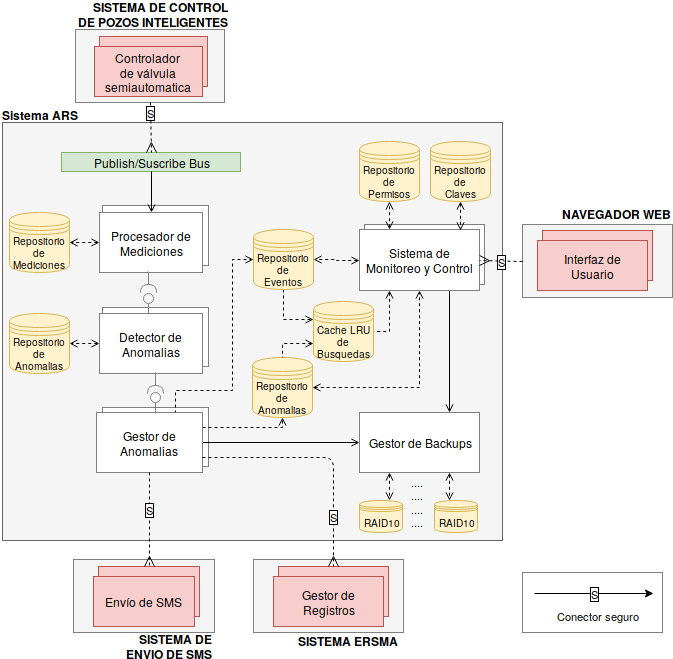
\includegraphics[scale=0.8]{figures/architecture.png}}
  \caption{Diagrama general de la arquitectura del sistema ARS de supervisión automática de yacimientos.}
\end{figure}

La arquitectura del Sistema ARS busca procesar los datos de alta frecuencia que son producidos por los diferentes controladores de válvula semiautomática del Sistema de Control de Pozos Inteligentes (SCPO). Cada controlador publica las mediciones de la válvula en un Publish/Suscribe Bus al que esta suscripto el componente de Procesamiento de Mediciones. El Procesador de Mediciones (sección \ref{procesador_mediciones}) básicamente se ocupa de transformar los datos de forma tal que puedan ser consumidos por el Detector de Anomalías.

El Detector de Anomalías (sección \ref{detector_anomalias}) identifica las diferentes anomalías en las mediciones, que son consumidas por el Gestor de Anomalías (sección \ref{gestor_anomalias}). Este componente notifica por SMS al Jefe de Operaciones del yacimiento de que se ha producido una anomalía, y a su vez guarda diferentes registros en los repositorios de Eventos y Anomalías para que luego puedan ser accedidos de forma externa. El componente también se comunica con un Gestor de Backups para garantizar la integridad de los datos ante casos de perdida o siniestros. Para cumplir con las normas internacionales, toda anomalía también es reportada a los organismos certificadores de calidad como el Ente Regulador de Seguridad Medio Ambiental (ERSMA). Para garantizar la confidencialidad de los datos, toda comunicación con un sistema externo es cifrada usando algoritmos simétricos y de clave publica/privada.

Todo usuario que queda acceder al Sistema de Informes de Eventos y al Sistema de Control y Monitoreo se debe autenticar por medio del Sistema de Usuarios. De esta forma los empleados del Ministerio y el Ente Regulador pueden acceder a los datos en todo momento.

\subsection{Procesamiento de mediciones}  \label{procesador_mediciones}

\begin{figure}[H]
  \resizebox{\textwidth}{!}{
    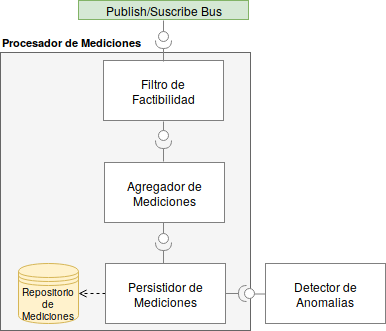
\includegraphics[scale=0.70]{figures/ProcesadorDeMediciones.png}
  }
  \caption{Diagrama de arquitectura de procesamiento de mediciones.}
\end{figure}

El Procesador de Mediciones consume datos de los diferentes controladores de válvula semiautomática de cada pozo a través de un Publish/Suscribe bus y una cola. Dada la alta frecuencia de los datos, no es factible ni practico guardarlos todos en una primera instancia antes de comenzar su procesamiento. Para reducir la cantidad de datos, primero se corre un Filtro de Factibilidad para remover los datos que no son realistas. Este filtro logra remover el 80\% de los datos espurios. Luego, los datos son agregados por el Agregador de Mediciones, el cual transforma los datos de alta frecuencia en datos en intervalos manejables de 15 minutos. Estos datos son luego consumidos por un Persistidor de Mediciones, que guarda los datos procesados y de menor dimensionalidad en un Repositorio de Mediciones. Estos datos también son enviados por medio de una cola al Detector de Anomalías.

Un dato que consideramos interesante explorar es la alta frecuencia de los datos. En caso de una caída del sistema, guardar los datos en un Repositorio luego del proceso de filtrado puede no ser relevante, dado que al momento en el que el sistema logra recuperarse rápidamente de una caída, datos muy similares van a ser incorporados desde los controladores de pozo inmediatamente, detectando posteriormente las mismas anomalías que hubiesen sido detectadas en caso de que el sistema hubiese funcionado correctamente.

\subsection{Detector de anomalías} \label{detector_anomalias}

\begin{figure}[H]
  \resizebox{\textwidth}{!}{
    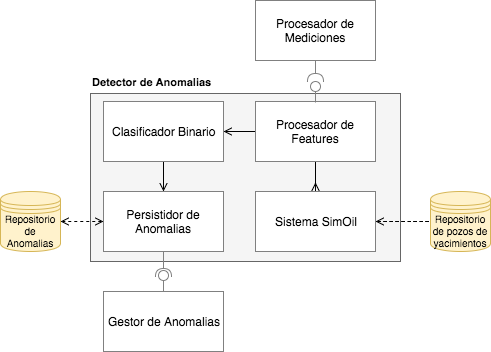
\includegraphics[scale=0.8]{figures/DetectorDeAnomalias.png}
  }
  \caption{Diagrama de arquitectura del detector de anomalías.}
\end{figure}

El Detector de Anomalías procesa los datos provistos por el Persistidor de Mediciones, arrancando con el Procesador de Features. Este componente extrae una serie de features o características con la asistencia del Sistema SimOil especificado en el trabajo anterior. Una vez procesados estos datos, se utiliza un clasificador binario (por el momento un modelo Logístico que ya esta entrenado) para definir si el dato procesado es o no una anomalía. En caso de ser una anomalía, se envía al Persistidor de Anomalías para bajar la probabilidad de perdida de datos ante un problema del sistema. Estos datos luego son enviados al Gestor de Anomalías.

\subsection{Gestor de anomalias} \label{gestor_anomalias}

\begin{figure}[H]
  \resizebox{\textwidth}{!}{
    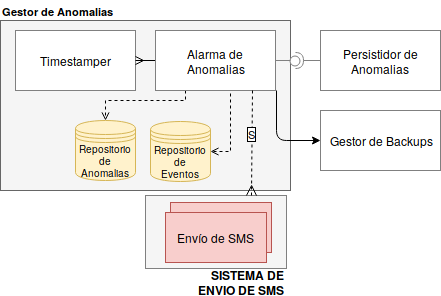
\includegraphics[scale=1]{figures/GestorDeAnomalias.png}
  }
  \caption{Diagrama de arquitectura del Gestor de Anomalías.}
\end{figure}

Al recibir datos de anomalías detectadas desde el Persistidor de Anomalías, la Alarma de Anomalías se ocupa de notificar al Jefe de Operaciones del correspondiente yacimiento de que se ha producido una anomalía. Luego a los datos se les asigna un timestamp y son guardados en el Repositorio de Anomalías y en el Repositorio de Eventos. Para lograr una mayor disponibilidad y tener un sistema tolerante a fallas, los datos sobre anomalías también son enviados a un Gestor de Backups que se ocupa mediante un conjunto de racks de RAIDs para tener mayor redundancia. En caso de falla, los procesos del componente se reinician y buscan los datos sobre las ultimas fallas que han ocurrido y no han sido reportadas desde este repositorio.

\subsection{Sistema de Monitoreo y Control} \label{gestor_anomalias}

\begin{figure}[H]
  \resizebox{\textwidth}{!}{
    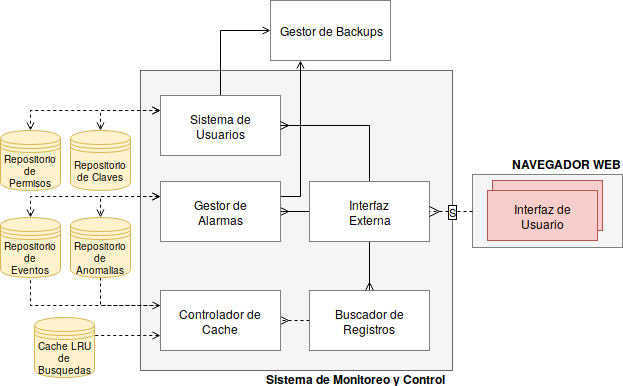
\includegraphics[scale=1]{figures/SistemaDeMonitoreoYControl.png}
  }
  \caption{Diagrama de arquitectura del Sistema de Monitoreo y Control.}
\end{figure}

\pagebreak

\subsection{¿Como satisface la arquitectura los atributos de calidad?}

A continuación explicaremos de forma mas explicita como la arquitectura propuesta satisface los atributos de calidad, tomando como punto de partida los escenarios especificados en la Sección \ref{cu}.

\subsubsection{Performance}
\subsubsection{Disponibilidad}
\subsubsection{Seguridad}
Hablar sobre el hecho de que alguien puede manipular los sensores de un pozo. Decir que se podría instalar un sistema biométrico para que solo personal autorizado tenga acceso a los sensores.

\subsubsection{Usabilidad}
\subsubsection{Modificabilidad}

\pagebreak

\section{Conclusiones}

Durante estos dos trabajos prácticos vimos distintos enfoques a la hora de diseñar software. Durante el primer trabajo utilizamos el diseño orientado a objetos (DOO), lo cual nos permitió realizar un diseño de más bajo nivel que el concebido mediante las diferentes arquitecturas del sistema (vista de C\&C + deployment). Con el DOO (programming in the small) pudimos diseñar reconociendo las distintas entidades de nuestro dominio del problema y convertirlas en objetos que se relacionan entre sí mediante envíos de mensajes. De esta manera es muy fácil implementar nuestra aplicación y comenzar a trabajar sobre ella. Este enfoque tiene algunas desventajas ya que no podemos ver algunos detalles como por ejemplo dónde van a correr nuestros procesos.

Para poder ver más otros detalles del sistema, entra en juego la arquitectura (programming in the large) que justamente viene a llenar ese vacío. La arquitectura nos permite ver las relaciones entre las distintas estructuras del sistema, y como se relacionan entre ellas, lo que resulta en una visión más abarcativa de la aplicación, no sólo porque nos permite definir las interacciones de nuestros procesos en tiempo de ejecución (mediante los diagramas de Componentes y Conectores) sino porque también nos permite identificar en dónde va a estar corriendo cada uno de esos procesos (mediante la vista de deployment).

Para concluir, el DOO es una muy buena forma de desarrollar módulos de la aplicación pero no es suficiente para desarrollar un buen sistema, ya que hay otro tipo de información relevante que no se puede visualizar con dichos módulos. Otra ventaja de las arquitecturas es que nos permite por medio de los escenarios de atributos de calidad proporcionarle al cliente un sistema que cumpla con los requerimientos no funcionales. Por esos motivos, es necesario construir arquitecturas usando el método de "programming in the large".

\end{document}
